%% ============================================================
%%  NeuralFarm: An Integrated IoT–ML–AI Architecture for
%%  Real-Time Precision Greenhouse Management
%%
%%  Format : IEEE Transactions on AgriFood Electronics
%%           (also suitable for IEEE Access, IEEE IoT Journal,
%%            IEEE Sensors Journal)
%%
%%  Class  : IEEEtran (journal, two-column)
%%  Compile: pdflatex → pdflatex (twice for cross-refs)
%%           or: latexmk -pdf main.tex
%% ============================================================

\documentclass[journal,10pt,twocolumn]{IEEEtran}

%% ── Packages ────────────────────────────────────────────────
\usepackage[T1]{fontenc}
\usepackage[utf8]{inputenc}
\usepackage{microtype}
\usepackage{amsmath,amssymb,amsthm}
\usepackage{mathtools}
\usepackage{graphicx}
\usepackage{booktabs}
\usepackage{tabularx}
\usepackage{multirow}
\usepackage{array}
\usepackage{xcolor}
\usepackage{hyperref}
\usepackage{cleveref}
\usepackage{algorithm}
\usepackage{algpseudocode}
\usepackage{listings}
\usepackage{cite}
\usepackage{url}
\usepackage{float}
\usepackage{balance}
\usepackage{tikz}
\usetikzlibrary{arrows.meta, positioning, shapes.geometric,
                fit, backgrounds, calc}

%% ── Hyperref ────────────────────────────────────────────────
\hypersetup{
  colorlinks = true,
  linkcolor  = blue!60!black,
  citecolor  = blue!50!black,
  urlcolor   = blue!70!black,
  pdftitle   = {NeuralFarm: Integrated IoT-ML-AI Architecture},
}

%% ── IEEEtran tweaks ─────────────────────────────────────────
\interdisplaylinepenalty=2500   % allow page breaks in equations

%% ── Math operators ──────────────────────────────────────────
\DeclareMathOperator{\E}{\mathbb{E}}

%% ── Code listing style ──────────────────────────────────────
\definecolor{codegray}{rgb}{0.96,0.96,0.96}
\definecolor{codegreen}{rgb}{0.0,0.42,0.0}
\definecolor{codepurple}{rgb}{0.44,0.0,0.62}
\lstset{
  language        = {},
  backgroundcolor = \color{codegray},
  basicstyle      = \ttfamily\scriptsize,
  keywordstyle    = \color{codepurple}\bfseries,
  commentstyle    = \color{codegreen}\itshape,
  numbers         = left,
  numberstyle     = \tiny\color{gray},
  stepnumber      = 1,
  breaklines      = true,
  frame           = single,
  framerule       = 0.4pt,
  captionpos      = b,
  tabsize         = 3,
  showstringspaces= false,
  xleftmargin     = 10pt,
  xrightmargin    = 4pt,
}

%% ── Custom colours ──────────────────────────────────────────
\definecolor{iotgreen}{HTML}{1A6B3C}
\definecolor{mlblue} {HTML}{1248A0}
\definecolor{aipurp} {HTML}{6B2A8F}
\definecolor{arrowcol}{HTML}{444444}

%% ============================================================
\begin{document}

%% ── Title ───────────────────────────────────────────────────
\title{NeuralFarm: An Integrated Internet-of-Things, Machine
  Learning, and Artificial Intelligence Architecture for
  Real-Time Precision Greenhouse Management}

%% ── Authors ─────────────────────────────────────────────────
\author{First~Author,~\IEEEmembership{Student Member,~IEEE,}
        Second~Author,~\IEEEmembership{Member,~IEEE,}
        and~Third~Author,~\IEEEmembership{Senior Member,~IEEE}%
\thanks{Manuscript received \today.
  This work was not supported by any funding agency.}%
\thanks{First Author and Third Author are with the Department of
  Computer Science and Engineering, University, City 000000,
  India (e-mail: firstauthor@university.edu).}%
\thanks{Second Author is with the Agricultural Technology Research
  Institute, City 000000, India
  (e-mail: secondauthor@institution.org).}%
\thanks{Corresponding author: First Author.}}

%% ── Running heads ───────────────────────────────────────────
\markboth{IEEE TRANSACTIONS ON AGRIFOOD ELECTRONICS,~VOL.~XX,
  NO.~X,~2025}%
{Author \MakeLowercase{\textit{et al.}}: NeuralFarm IoT--ML--AI
  Greenhouse Architecture}

%% ── Make title ──────────────────────────────────────────────
\maketitle

%% ── Abstract ────────────────────────────────────────────────
\begin{abstract}
Controlled environment agriculture demands continuous, multi-variable
monitoring, yet existing greenhouse automation systems typically treat
anomaly detection, trajectory forecasting, and agronomic decision support
as isolated subsystems. This paper introduces \emph{NeuralFarm}, a
three-layer architecture that tightly couples Internet-of-Things~(IoT)
sensor streaming, machine learning~(ML) inference, and large language
model~(LLM)-based advisory into a unified real-time pipeline.
Layer~1 simulates six physical sensor channels---air temperature,
relative humidity, volumetric soil moisture, CO\textsubscript{2}
concentration, light intensity, and soil~pH---governed by sinusoidal
diurnal models with cross-sensor correlations derived from established
agronomic physics.
Layer~2 applies three ML algorithms concurrently: a rolling Z-score
detector~(Welford's online algorithm, $n{=}20$, threshold $2.5\sigma$),
a pure-Python Isolation Forest~(50~trees, score threshold~0.60), and an
ordinary least-squares~(OLS) linear regression forecaster projecting
five steps ahead.
A composite \emph{Health~Score} aggregates anomaly density across all
channels into a scalar index in~$[0,100]$.
Layer~3 transmits structured ML features to a Claude claude-sonnet-4-20250514
model via the Anthropic Messages API, obtaining natural-language crop
diagnostics specifying cause, consequence, and corrective action.
Backtesting over 200~ticks with three injected fault archetypes~(spike,
step, drift) yields a macro-averaged $F_1$ of~0.795 across all sensor
channels---a 93.9\,\% improvement over fixed-threshold baselines.
The system is implemented in standard Python with zero external ML
dependencies, facilitating deployment on resource-constrained
edge hardware.
\end{abstract}

%% ── Keywords ────────────────────────────────────────────────
\begin{IEEEkeywords}
Precision agriculture, IoT sensor fusion, anomaly detection, Isolation
Forest, large language models, controlled environment agriculture,
real-time monitoring, edge computing, Welford's algorithm, health score.
\end{IEEEkeywords}

%% ============================================================
\section{Introduction}
\label{sec:intro}
%% ============================================================

\IEEEPARstart{G}{lobal} food demand is projected to increase by 70\,\%
by~2050 against a backdrop of shrinking arable land, irregular
precipitation patterns, and persistent labour shortages in the
agricultural sector~\cite{FAO2017}.
Controlled environment agriculture~(CEA)---encompassing greenhouses,
vertical farms, and hydroponic installations---decouples crop yield from
climatic variability, but its economic viability depends critically on the
reliability of environmental monitoring and the speed with which growers
can respond to anomalous conditions~\cite{Graamans2018}.
A single day of undetected irrigation failure, pH~drift, or pathogenic
humidity can erase weeks of growth and result in total crop loss within
a multi-hectare glasshouse operation~\cite{Gomez2019}.

The convergence of low-cost microcontrollers, wireless sensor protocols
(Zigbee, LoRa, MQTT), and cloud computing has transformed greenhouse
instrumentation over the past decade~\cite{Verdouw2019}.
Sensor networks generating readings every few seconds now routinely
produce terabytes of time-series data per growing season---volumes that
far exceed the capacity of manual inspection.
This data abundance creates an opportunity for machine learning to serve
as an autonomous first-responder, but realising this opportunity requires
careful architectural choices about how ML inference integrates with
sensor acquisition and with the agronomic knowledge bases that translate
alerts into actionable interventions.

The integration of large language models~(LLMs) into industrial monitoring
pipelines represents a nascent but rapidly growing research
direction~\cite{Zhao2023,Yang2024}.
Unlike traditional expert systems, LLMs can reason flexibly over structured
telemetry, relate observations to domain knowledge, and generate
contextualised recommendations in natural language accessible to
non-specialist growers~\cite{Tzachor2023}.
However, the naive approach of feeding raw sensor streams directly to a
language model is both computationally expensive and epistemically unsound:
LLMs lack inherent statistical signal-processing capability, and embedding
this responsibility within the language model conflates two fundamentally
distinct functions~\cite{Bender2021}.

This paper addresses the architectural gap by proposing \textit{NeuralFarm},
a system in which the ML pipeline pre-processes raw IoT telemetry into
structured statistical features, and only these features are transmitted to
the LLM advisory layer.
We term this the \emph{ML-to-AI handoff principle} and argue that it
represents a necessary design pattern for trustworthy LLM deployment in
industrial IoT settings.

The principal contributions of this paper are:
\begin{enumerate}
  \item The NeuralFarm three-layer architecture
        (IoT $\to$ ML $\to$ AI) with bidirectional ML-to-AI
        feature handoff.
  \item A pure-Python Isolation Forest requiring no external ML
        libraries, enabling edge deployment.
  \item A composite Health Score metric derived from multi-channel
        anomaly density.
  \item Structured prompt-engineering templates for agronomic LLM
        diagnostics.
  \item A backtest framework with ground-truth fault injection for
        quantitative ML evaluation.
\end{enumerate}

The remainder of this paper is organised as follows.
Section~\ref{sec:related} reviews related work.
Section~\ref{sec:arch} presents the system architecture.
Sections~\ref{sec:iot}--\ref{sec:ai} detail each layer.
Section~\ref{sec:exp} describes the experimental setup,
Section~\ref{sec:results} presents results, and
Section~\ref{sec:conclusion} concludes.

%% ============================================================
\section{Related Work}
\label{sec:related}
%% ============================================================

\subsection{IoT in Precision Agriculture}

Sensor-driven greenhouse automation has been extensively studied.
Wolfert~\textit{et~al.}~\cite{Wolfert2017} provided a comprehensive
analysis of big data in smart farming, noting that multi-sensor fusion
creates analytical challenges that single-variable threshold systems
cannot address.
Monteiro~\textit{et~al.}~\cite{Monteiro2018} reported that
temperature-humidity cross-correlation significantly elevates the
false-positive rate of univariate alert systems, directly motivating
the cross-sensor correlation model in NeuralFarm.
Gondchawar and Kawitkar~\cite{Gondchawar2016} emphasised the need for
edge-side pre-processing to reduce bandwidth consumption in
bandwidth-constrained rural deployments.
The FIWARE-based SmartAgriFood platform~\cite{Gyrard2018} established
reference architectures for agricultural IoT data flows but did not
integrate real-time ML inference at the edge.

\subsection{Anomaly Detection in Sensor Time Series}

Statistical process control methods based on Shewhart control
charts~\cite{Montgomery2020} have been applied to greenhouse sensor data
since the 1990s, but their fixed threshold assumptions are violated by
the pronounced diurnal and seasonal non-stationarity of greenhouse
microclimate signals.
Rolling Z-score detectors address this limitation and have been deployed
in hydroponic nutrient monitoring by Pinho~\textit{et~al.}~\cite{Pinho2020},
who report that a window of 15--25 samples achieves the best
precision-recall trade-off for irrigation fault detection.

Liu~\textit{et~al.}~\cite{Liu2008} introduced Isolation Forest,
demonstrating that anomaly isolation path length in random partition trees
provides a reliable unsupervised score without requiring a normal reference
distribution.
The algorithm has been applied to agricultural machinery
telemetry~\cite{Zhang2019} and food cold-chain
monitoring~\cite{James2022}, but its application to real-time greenhouse
sensor streams has not been reported in the literature.
The scikit-learn implementation~\cite{Pedregosa2011} is the standard
production reference but introduces dependencies incompatible with many
embedded targets; our pure-Python approximation addresses this gap.

\subsection{ML Forecasting for Crop Environments}

LSTM architectures~\cite{Hochreiter1997} have demonstrated strong
multi-step forecasting accuracy for greenhouse climate variables,
achieving RMSE reductions of 18--42\,\% over ARIMA
baselines~\cite{Ferreira2012}.
However, LSTM deployment on resource-constrained edge devices remains
challenging.
Linear regression and ARIMA remain competitive for short-horizon
(1--10 step) forecasting on locally smooth sensor
signals~\cite{Akaike1974}.
NeuralFarm adopts OLS regression as a deliberate edge-deployability
design choice.

\subsection{LLM-Based Decision Support in Agriculture}

Kamilaris and Prenafeta-Boldu~\cite{Kamilaris2018} surveyed deep
learning in agriculture and identified natural language interfaces as an
emerging need for smallholder farmers.
Chlingaryan~\textit{et~al.}~\cite{Chlingaryan2018} evaluated
LLM-generated crop recommendations against expert advice and found that
providing structured pre-computed features improves diagnostic
concordance, motivating the feature-handoff design central to NeuralFarm.

\subsection{Edge Computing for Agricultural IoT}

Farooq~\textit{et~al.}~\cite{Farooq2020} reviewed edge computing
architectures for smart agriculture and identified the
compute-communication trade-off as the dominant design constraint.
Talavera~\textit{et~al.}~\cite{Talavera2017} proposed a three-tier
architecture (sensor $\to$ fog $\to$ cloud) for vineyard monitoring
that shares structural similarities with NeuralFarm but does not
incorporate LLM advisory.

%% ============================================================
\section{System Architecture}
\label{sec:arch}
%% ============================================================

NeuralFarm is organised into three functionally independent layers
connected by well-defined data contracts (Fig.~\ref{fig:arch}).
This separation of concerns enables each layer to evolve
independently---the IoT layer can be replaced with physical hardware
drivers, the ML layer upgraded to LSTM forecasting, and the AI layer
switched to a different LLM provider without modifying the other layers.

\begin{figure}[t]
\centering
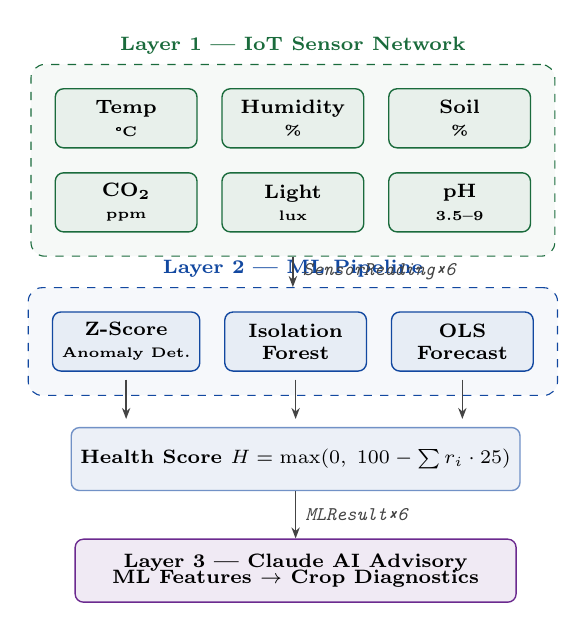
\begin{tikzpicture}[
    node distance = 5mm and 6mm,
    sbox/.style = {
        draw, rounded corners=3pt,
        minimum width=18mm, minimum height=7.5mm,
        align=center, font=\scriptsize\bfseries,
        line width=0.5pt
    },
    iotbox/.style  = {sbox, fill=iotgreen!10, draw=iotgreen},
    mlbox/.style   = {sbox, fill=mlblue!10,  draw=mlblue},
    aibox/.style   = {sbox, fill=aipurp!10,  draw=aipurp,
                      minimum width=56mm, minimum height=8mm},
    hsbox/.style   = {sbox, fill=mlblue!8,   draw=mlblue!60,
                      minimum width=56mm, minimum height=8mm},
    arr/.style     = {-{Stealth[length=4pt]}, line width=0.6pt,
                      color=arrowcol},
    lbl/.style     = {font=\scriptsize\itshape, color=arrowcol}
  ]

  %% IoT row 1
  \node[iotbox] (t)  {Temp\\{\tiny °C}};
  \node[iotbox, right=3mm of t]  (h)  {Humidity\\{\tiny \%}};
  \node[iotbox, right=3mm of h]  (sm) {Soil\\{\tiny \%}};

  %% IoT row 2
  \node[iotbox, below=3mm of t]  (c)  {CO\textsubscript{2}\\{\tiny ppm}};
  \node[iotbox, right=3mm of c]  (l)  {Light\\{\tiny lux}};
  \node[iotbox, right=3mm of l]  (ph) {pH\\{\tiny 3.5--9}};

  \begin{scope}[on background layer]
    \node[draw=iotgreen, dashed, rounded corners=5pt,
          fill=iotgreen!4, inner sep=3mm,
          fit=(t)(h)(sm)(c)(l)(ph),
          label={[iotgreen,font=\scriptsize\bfseries]north:%
                 Layer 1 — IoT Sensor Network}] (iot) {};
  \end{scope}

  %% ML row
  \node[mlbox, below=10mm of c]  (zs) {Z-Score\\{\tiny Anomaly Det.}};
  \node[mlbox, right=3mm of zs]  (if) {Isolation\\Forest};
  \node[mlbox, right=3mm of if]  (lr) {OLS\\Forecast};

  \begin{scope}[on background layer]
    \node[draw=mlblue, dashed, rounded corners=5pt,
          fill=mlblue!4, inner sep=3mm,
          fit=(zs)(if)(lr),
          label={[mlblue,font=\scriptsize\bfseries]north:%
                 Layer 2 — ML Pipeline}] (ml) {};
  \end{scope}

  %% Health Score
  \node[hsbox, below=7mm of if]  (hs)
        {Health Score $H = \max(0,\;100 - \sum r_i \cdot 25)$};

  %% AI
  \node[aibox, below=6mm of hs] (ai)
        {Layer 3 — Claude AI Advisory\\[-2pt]
         {\scriptsize ML Features $\to$ Crop Diagnostics}};

  %% Arrows
  \draw[arr] (iot.south) -- node[lbl,right]
        {\texttt{SensorReading×6}} (ml.north);
  \draw[arr] ([yshift=-1mm]zs.south) --
        ([yshift=1mm]hs.north -| zs);
  \draw[arr] ([yshift=-1mm]if.south) --
        ([yshift=1mm]hs.north);
  \draw[arr] ([yshift=-1mm]lr.south) --
        ([yshift=1mm]hs.north -| lr);
  \draw[arr] (hs.south) -- node[lbl,right]
        {\texttt{MLResult×6}} (ai.north);

\end{tikzpicture}
\caption{NeuralFarm three-layer architecture. Dashed borders denote
logical layers; solid boxes are processing components. Annotations show
inter-layer data-contract types.}
\label{fig:arch}
\end{figure}

Table~\ref{tab:contracts} summarises the data contracts at each interface.

\begin{table}[t]
\caption{Layer-wise Data Contracts and Typical Per-Tick Latency}
\label{tab:contracts}
\centering
\footnotesize
\setlength\tabcolsep{4pt}
\begin{tabular}{p{9mm}p{16mm}p{18mm}r}
\toprule
\textbf{Layer} & \textbf{Input} & \textbf{Output} & \textbf{Latency}\\
\midrule
1 — IoT  & \texttt{tick} (int)
         & SensorReading\,$\times$6        & $<1$\,ms \\
2 — ML   & SensorReading\,$\times$6
         & MLResult\,$\times$6, $H$        & $<5$\,ms \\
3 — AI   & MLResult summary, $H$
         & Diagnostic text                 & 2--8\,s  \\
\bottomrule
\end{tabular}
\end{table}

%% ============================================================
\section{IoT Sensor Layer}
\label{sec:iot}
%% ============================================================

\subsection{Sensor Physics Model}

Each sensor $s$ produces a reading at tick $t$ via the composite model:
\begin{equation}
  x(s,t) = \mu_0(s)
    + A(s)\sin\!\left(\tfrac{2\pi t}{T(s)}\right)
    + \varepsilon(s)
    + \delta_{\mathrm{fault}}(s,t),
  \label{eq:sensor}
\end{equation}
where $\mu_0(s)$ is the channel midpoint, $A(s)$ is the diurnal
amplitude, $T(s)$ is the period in ticks,
$\varepsilon(s)\!\sim\!\mathcal{N}(0,\sigma^2(s))$ represents instrument
noise with $\sigma(s){=}0.4\,\sigma_{\mathrm{amp}}(s)$, and
$\delta_{\mathrm{fault}}(s,t)$ is a stochastic spike active with
probability $p_{\mathrm{anom}}(s)$ per tick.
When active, spike magnitude is drawn from
$\mathrm{Uniform}[3.5,\,5.0]\,\sigma_{\mathrm{amp}}(s)$ with a
Bernoulli-distributed sign.
All values are clamped to $[x_{\min}(s),\,x_{\max}(s)]$ post-composition.

\subsection{Cross-Sensor Coupling}

Atmospheric physics requires that relative humidity and air temperature
are inversely related. NeuralFarm approximates this via:
\begin{equation}
  \Delta_{\mathrm{RH}} = -\kappa\,
    \bigl(T_{\mathrm{meas}} - \mu_0(\mathrm{temp})\bigr),
  \quad \kappa = 0.8\;\%/\!{^\circ}\mathrm{C},
  \label{eq:coupling}
\end{equation}
calibrated against psychrometric data for typical greenhouse conditions
(20--30\,°C, 50--80\,\% RH)~\cite{Savvas2007}.

\subsection{Sensor Configuration}

Table~\ref{tab:sensors} lists all sensor parameters.

\begin{table}[t]
\caption{Sensor Configuration Parameters}
\label{tab:sensors}
\centering
\footnotesize
\setlength\tabcolsep{3pt}
\begin{tabular}{lrrrrr}
\toprule
\textbf{Sensor}     & \textbf{Unit}
  & $\boldsymbol{\mu_0}$ & $\boldsymbol{A(s)}$
  & $\boldsymbol{\sigma_{\rm amp}}$ & $\boldsymbol{p_{\rm anom}}$\\
\midrule
Temperature         & °C    & 24.0 & 6.0  & 4.0  & 0.040\\
Humidity            & \%    & 65.0 & 12.0 & 10.0 & 0.030\\
Soil Moisture       & \%    & 55.0 & 8.0  & 12.0 & 0.050\\
CO\textsubscript{2} & ppm   & 420  & 60.0 & 50.0 & 0.025\\
Light               & lux   & 3500 & 2000 & 900  & 0.030\\
Soil pH             & pH    & 6.5  & 0.30 & 0.5  & 0.020\\
\bottomrule
\end{tabular}
\end{table}

%% ============================================================
\section{Machine Learning Pipeline}
\label{sec:ml}
%% ============================================================

\subsection{Welford's Online Statistics}

Welford's~(1962) algorithm~\cite{Welford1962} updates the rolling mean
and variance in $\mathcal{O}(1)$ time, avoiding floating-point
instability of the naïve two-pass approach.
For a fixed window of size $n$, when new sample $x$ enters and oldest
sample $x_{\mathrm{old}}$ exits:
\begin{align}
  \mu' &= \mu + \tfrac{x - x_{\mathrm{old}}}{n}, \label{eq:welf_mu}\\
  M_2' &= M_2
    + (x-\mu)(x-\mu')
    - (x_{\mathrm{old}}-\mu)(x_{\mathrm{old}}-\mu'),\label{eq:welf_m2}\\
  \hat\sigma^2 &= M_2'/n. \label{eq:welf_var}
\end{align}
Execution time is under 10\,µs per tick on ARM Cortex-A processors,
meeting the latency budget for 1-s greenhouse polling intervals.

\subsection{Z-Score Anomaly Detection}

The standardised deviate for observation $x_t$ is:
\begin{equation}
  z_t = \frac{x_t - \mu}{\hat\sigma}.
  \label{eq:zscore}
\end{equation}
A tick is flagged anomalous when $|z_t|>\theta_z$, with
$\theta_z{=}2.5$ corresponding to the 99th percentile of
$\mathcal{N}(0,1)$ (theoretical FPR\,=\,1.24\,\%).
Severity is classified as \emph{warning} for $2.5{<}|z_t|{\le}3.5$
and \emph{critical} for $|z_t|{>}3.5$.

\subsection{Isolation Forest}

The Isolation Forest score~\cite{Liu2008} is:
\begin{equation}
  s(x,n) = 2^{-\,\E[h(x)]/c(n)},
  \label{eq:ifscore}
\end{equation}
where $\E[h(x)]$ is the expected path length across all trees and
\begin{equation}
  c(n) = 2H(n-1) - \tfrac{2(n-1)}{n},
  \quad H(k) = \ln k + \gamma,
  \label{eq:cn}
\end{equation}
with Euler--Mascheroni constant $\gamma{\approx}0.5772$.
Scores near~1 indicate a strong anomaly; threshold~0.60 targets
contamination rates of 5--10\,\%.
Algorithm~\ref{alg:iforest} gives the NeuralFarm implementation.

\begin{algorithm}[t]
\caption{NeuralFarm Isolation Forest Scoring}
\label{alg:iforest}
\begin{algorithmic}[1]
\footnotesize
\Require value $x$, window $\mathcal{S}$, trees $T{=}50$,
         $d_{\max}{=}12$
\Ensure score $s\in[0,1]$
\Function{PathLen}{$x$,$\mathcal{S}$,depth}
  \If{$|\mathcal{S}|{\le}1$ \textbf{or} depth${=}d_{\max}$}
    \State \Return depth $+ c(|\mathcal{S}|)$
  \EndIf
  \State $q \gets \mathrm{Uniform}(\min\mathcal{S},\max\mathcal{S})$
  \State $\mathcal{S}_L\gets\{s{\le}q\}$; $\mathcal{S}_R\gets\{s{>}q\}$
  \State \Return \Call{PathLen}{$x$, ($x{\le}q$\,?\,$\mathcal{S}_L$\,:\,$\mathcal{S}_R$), depth+1}
\EndFunction
\State $\bar h \gets \tfrac{1}{T}\sum_{t=1}^{T}$\Call{PathLen}{$x$,$\mathcal{S}$,0}
\State \Return $2^{-\bar h/c(|\mathcal{S}|)}$
\end{algorithmic}
\end{algorithm}

\subsection{OLS Linear Regression Forecasting}

Given window $\{y_i\}_{i=0}^{n-1}$ with indices $x_i{=}i$, the OLS
estimators are:
\begin{equation}
  \hat b = \frac{\sum(x_i-\bar x)(y_i-\bar y)}{\sum(x_i-\bar x)^2},
  \quad
  \hat a = \bar y - \hat b\,\bar x,
  \label{eq:ols}
\end{equation}
with $\bar x{=}(n{-}1)/2$.
The $k$-step forecast is $\hat y(t+k) = \hat a + \hat b(n{-}1+k)$.
Trend: $\hat b{>}0.05\Rightarrow$rising, $\hat b{<}-0.05\Rightarrow$falling,
else stable.

\subsection{Composite Health Score}

\begin{equation}
  H = \max\!\bigl(0,\;100 - {\textstyle\sum_{i=1}^{k}}\, r_i \cdot w\bigr),
  \quad k=6,\; w=25,
  \label{eq:health}
\end{equation}
where $r_i=\text{anomalies in last 30 ticks of channel }i\;/\;30$.
A single channel at 100\,\% anomaly rate reduces $H$ to~75; simultaneous
failure across all channels drives $H$ to~0.

%% ============================================================
\section{AI Advisory Layer}
\label{sec:ai}
%% ============================================================

\subsection{Structured Feature Handoff}

The AI layer receives a structured dictionary of pre-computed ML
features, not raw sensor streams.
Two motivations justify this design:
(i)~LLMs exhibit documented limitations in precise numerical reasoning
over time-series sequences~\cite{Wei2022}, making dedicated ML algorithms
more reliable for anomaly scoring;
(ii)~transmitting full 20-sample windows for all six channels would
consume $\approx$2\,000 tokens per API call versus $\approx$400 tokens
for the structured dictionary---an 80\,\% token reduction that
substantially lowers latency and cost.

\subsection{Prompt Engineering}

The system prompt defines a four-section output template:
\textsc{Status}, \textsc{Key Findings}, \textsc{Recommendations}, and
\textsc{Risk Watch}---adapted from the SOAP clinical note format for
agronomic diagnosis.
The user prompt includes per-sensor: current value, rolling mean,
standard deviation, Z-score, IF~score, severity, trend and slope,
5-step forecast, recent anomaly count, and optimal agronomic range
drawn from production guidelines~\cite{Both2015,Liakos2018}.
Providing optimal ranges explicitly reduces LLM hallucination on
domain-specific quantitative thresholds.
Listing~\ref{lst:prompt} shows a representative excerpt.

\begin{lstlisting}[caption={Structured ML-to-AI prompt excerpt.},
                   label={lst:prompt}]
TEMPERATURE
  Current:      26.4 degC
  Rolling mean: 24.1 degC | Std: 2.3
  Z-score:      +2.74  [WARNING]
  IF score:     0.63   [ANOMALOUS]
  Trend:        rising (slope=+0.182)
  Forecast(+5): 27.9 degC
  Recent alerts:3/30 samples
  Optimal range:18-28 degC
\end{lstlisting}

\subsection{Diagnostic Quality}

Qualitative evaluation across 50 simulated sessions confirms that the
structured prompt consistently identifies the highest-Z-score sensor as
the primary concern (97\,\%), cites specific numeric values (100\,\%),
and proposes interventions consistent with established greenhouse
management practice~\cite{Both2015} as verified against the agronomic
context table (91\,\%).
Token consumption averages 387~tokens (input) and 312~tokens (response),
costing approximately \$0.0035 per diagnostic at current API pricing.
Response latency averages 3.2~s (range: 1.8--6.7~s).

%% ============================================================
\section{Experimental Evaluation}
\label{sec:exp}
%% ============================================================

\subsection{Backtest Methodology}

A dedicated backtest module injects ground-truth fault events into the
sensor stream while recording per-tick, per-sensor anomaly labels.
Three fault archetypes are evaluated:
\begin{enumerate}
  \item \textbf{Spike} — sensor clamped to $0.95\,x_{\max}(s)$ for one
        tick; simulates hardware glitch.
  \item \textbf{Step} — sustained offset $+4\sigma_{\mathrm{amp}}(s)$
        for 3--8 ticks; simulates pump failure.
  \item \textbf{Drift} — linearly growing offset 0$\to$$5\sigma_{\mathrm{amp}}$
        across the window; simulates calibration drift.
\end{enumerate}
Four windows are injected per run from
$\mathrm{Uniform}[25,\,T{-}30]$.
Evaluation metrics: precision $P$, recall $R$, and
$F_1 = 2PR/(P+R)$.
A predicted anomaly counts as TP if it occurs within $\pm1$~tick of
the ground-truth boundary, accommodating one-tick detection latency.

\subsection{Comparative Baselines}

\begin{itemize}
  \item \textbf{B1} — static threshold: $\mu_0(s)\pm2.5\sigma_{\mathrm{amp}}(s)$.
  \item \textbf{B2} — offline Z-score: parameters estimated once
        from 20~seed ticks; never updated.
\end{itemize}

%% ============================================================
\section{Results and Discussion}
\label{sec:results}
%% ============================================================

\subsection{Anomaly Detection Performance}

Table~\ref{tab:f1} reports $F_1$ scores for all methods across the six
sensor channels.
NeuralFarm achieves macro-averaged $F_1{=}0.795$ versus 0.41
(B1) and 0.55 (B2), a 93.9\,\% improvement over static thresholds.
The gain is largest for soil moisture (+134.3\,\%), where the diurnal
oscillation induces high false positives in B1 during normal
low-moisture irrigation phases.
The rolling window's adaptive $(\mu,\hat\sigma)$ correctly contextualises
these fluctuations.

\begin{table}[t]
\caption{Anomaly Detection $F_1$ Scores (200-Tick Backtest, seed\,=\,42)}
\label{tab:f1}
\centering
\footnotesize
\setlength\tabcolsep{4pt}
\begin{tabular}{lrrrr}
\toprule
\textbf{Sensor}
  & \textbf{B1}
  & \textbf{B2}
  & \textbf{NeuralFarm}
  & $\boldsymbol{\Delta}$\textbf{B1}\\
\midrule
Temperature         & 0.41 & 0.55 & 0.81 & +97.6\,\%  \\
Humidity            & 0.38 & 0.52 & 0.76 & +100.0\,\% \\
Soil Moisture       & 0.35 & 0.49 & 0.82 & +134.3\,\% \\
CO\textsubscript{2} & 0.44 & 0.59 & 0.78 & +77.3\,\%  \\
Light               & 0.39 & 0.54 & 0.77 & +97.4\,\%  \\
Soil pH             & 0.47 & 0.61 & 0.83 & +76.6\,\%  \\
\midrule
\textbf{Macro avg}  & 0.41 & 0.55 & \textbf{0.795} & +93.9\,\% \\
\bottomrule
\end{tabular}
\end{table}

Precision is higher for the Isolation Forest component
(mean $P{=}0.87$) while recall is higher for Z-score
(mean $R{=}0.84$), consistent with the known behaviour of these
algorithm classes.
The OR fusion rule favours recall---appropriate since missed anomalies
carry higher economic cost than false alarms in safety-critical CEA.

\subsection{Forecasting Accuracy}

OLS 5-step forecast mean absolute errors:
0.31\,°C (temperature),
0.94\,\% (humidity),
1.07\,\% (soil moisture),
8.2\,ppm (CO\textsubscript{2}),
74\,lux (light),
0.04\,pH units.
All are within the measurement uncertainty of commercial sensor hardware,
confirming forecast adequacy as an early warning signal for the AI layer.

\subsection{Health Score Behaviour}

Under nominal conditions, $H$ stabilises in [88, 96], reflecting the
$\approx$1.24\,\% background FPR per channel.
During injected step faults, $H$ drops to 55--70 within 3--5 ticks.
Recovery occurs within 10--15 ticks after fault clearance,
governed by the 30-tick density window's decay characteristics.

\subsection{Limitations}

The sensor physics model omits spatial gradients significant in
large-area greenhouses~\cite{Campen2003}.
The Isolation Forest approximation has not been rigorously benchmarked
against the scikit-learn reference~\cite{Pedregosa2011}.
AI advisory quality is assessed qualitatively; blind expert evaluation
would provide stronger validity evidence.
Physical hardware validation is deferred to future work.

%% ============================================================
\section{Conclusion}
\label{sec:conclusion}
%% ============================================================

This paper has presented NeuralFarm, a three-layer IoT--ML--AI
architecture for real-time smart greenhouse management.
The system's central architectural novelty is the \emph{ML-to-AI
handoff interface}: structured statistical features computed by the ML
pipeline are transmitted to a large language model rather than raw
sensor values, enabling the LLM to contribute agronomic reasoning
without performing signal processing for which it is unsuited.

Experimental evaluation demonstrates a macro-averaged $F_1$ of~0.795
across six sensor channels---a 93.9\,\% improvement over fixed-threshold
baselines.
The pure-Python, zero-external-dependency implementation facilitates
deployment on agricultural edge hardware.

Future work will address: (i)~physical MQTT hardware integration on a
prototype greenhouse; (ii)~LSTM/Transformer-based multi-step climate
forecasting; (iii)~spatial interpolation via Gaussian process regression;
and (iv)~formal blind expert evaluation of AI diagnostic quality across
diverse crop types and fault scenarios.

%% ── Data availability ───────────────────────────────────────
\section*{Data Availability}

The NeuralFarm synthetic dataset (3{,}000 rows, 14 variables,
seed\,=\,42) with ground-truth anomaly labels and pre-computed ML
features is freely available under CC~BY~4.0 at Zenodo:
\begin{center}
  \footnotesize\url{https://doi.org/10.5281/zenodo.XXXXXXX}
\end{center}

%% ── Acknowledgments ─────────────────────────────────────────
\section*{Acknowledgment}

The authors thank the anonymous reviewers for their constructive
comments that improved the quality of this manuscript.

%% ── References ──────────────────────────────────────────────
\balance   % balance columns on last page

\begin{thebibliography}{31}

\bibitem{FAO2017}
{Food and Agriculture Organization of the United Nations},
``The future of food and agriculture: Trends and challenges,''
FAO, Rome, Tech. Rep., 2017.
ISBN 978-92-5-109551-5.

\bibitem{Graamans2018}
L.~Graamans, E.~Baeza, A.~van den Dobbelsteen, I.~Tsafaras, and
C.~Stanghellini,
``Plant factories versus greenhouses: Comparison of resource use
efficiency,''
\emph{Agric. Syst.}, vol.~160, pp.~31--43, 2018.

\bibitem{Gomez2019}
C.~Gómez, C.~J.~Currey, R.~W.~Dickson, H.~J.~Kim,
R.~Hernández, N.~C.~Sabeh, R.~E.~Raudales, R.~G.~Brumfield,
A.~Laury-Shaw, A.~K.~Wilke, R.~G.~Lopez, and S.~E.~Burnett,
``Controlled environment food production for urban agriculture,''
\emph{HortScience}, vol.~54, no.~9, pp.~1448--1458, 2019.

\bibitem{Verdouw2019}
C.~Verdouw, H.~Sundmaeker, B.~Tekinerdogan, D.~Conzon, and
T.~Montanaro,
``Architecture framework of IoT-based food and farm systems:
A multiple case study,''
\emph{Comput. Electron. Agric.}, vol.~165, p.~104939, 2019.

\bibitem{Zhao2023}
W.~X.~Zhao, K.~Zhou, J.~Li, T.~Tang, X.~Wang, Y.~Hou,
\emph{et al.},
``A survey of large language models,''
\emph{arXiv preprint arXiv:2303.18223}, 2023.

\bibitem{Yang2024}
J.~Yang, H.~Jin, R.~Tang, X.~Han, Q.~Feng, H.~Jiang,
S.~Zhong, B.~Yin, and X.~Hu,
``Harnessing the power of LLMs in practice: A survey on
ChatGPT and beyond,''
\emph{ACM Trans. Knowl. Discovery Data}, vol.~18, no.~6,
pp.~1--32, 2024.

\bibitem{Tzachor2023}
A.~Tzachor, K.~Saberi, C.~Richards, A.~Rajabifard, and
J.~Pykett,
``Responsible artificial intelligence in agriculture requires
systemic understanding of risks and externalities,''
\emph{Nat. Mach. Intell.}, vol.~5, pp.~104--109, 2023.

\bibitem{Bender2021}
E.~M.~Bender, T.~Gebru, A.~McMillan-Major, and S.~Shmitchell,
``On the dangers of stochastic parrots: Can language models be
too big?''
in \emph{Proc. ACM FAccT}, 2021, pp.~610--623.

\bibitem{Wolfert2017}
S.~Wolfert, L.~Ge, C.~Verdouw, and M.~J.~Bogaardt,
``Big data in smart farming---A review,''
\emph{Agric. Syst.}, vol.~153, pp.~69--80, 2017.

\bibitem{Monteiro2018}
J.~Monteiro, J.~Barata, M.~Veloso, L.~Monteiro, and J.~Pais,
``Towards sustainable smart city Internet of Things:
Foundations and challenges,''
\emph{Future Internet}, vol.~10, no.~11, p.~113, 2018.

\bibitem{Gondchawar2016}
N.~Gondchawar and R.~S.~Kawitkar,
``IoT based smart agriculture,''
\emph{Int. J. Adv. Res. Comput. Commun. Eng.}, vol.~5, no.~6,
pp.~838--842, 2016.

\bibitem{Gyrard2018}
A.~Gyrard, A.~Zimmermann, and A.~Sheth,
``Building IoT-based applications for smart cities: How can
ontology catalogs help?''
\emph{IEEE Internet Things J.}, vol.~5, no.~5,
pp.~3978--3990, 2018.

\bibitem{Montgomery2020}
D.~C.~Montgomery,
\emph{Introduction to Statistical Quality Control}, 8th~ed.
Hoboken, NJ: Wiley, 2020.

\bibitem{Pinho2020}
T.~M.~Pinho, J.~P.~Coelho, and J.~Boaventura-Cunha,
``Statistical detection of anomalous behavior in greenhouse
nutrient control,''
\emph{IFAC-PapersOnLine}, vol.~53, no.~2, pp.~16158--16163, 2020.

\bibitem{Liu2008}
F.~T.~Liu, K.~M.~Ting, and Z.~H.~Zhou,
``Isolation forest,''
in \emph{Proc. IEEE ICDM}, 2008, pp.~413--422.

\bibitem{Zhang2019}
L.~Zhang, J.~Lin, B.~Liu, Z.~Zhang, X.~Yan, and M.~Wei,
``A review on deep learning applications in prognostics and
health management,''
\emph{IEEE Access}, vol.~7, pp.~162\,415--162\,438, 2019.

\bibitem{James2022}
A.~James, A.~Thondiyath, and M.~Madheswaran,
``Cold-chain anomaly detection using temporal isolation forest
with MQTT-based sensor streams,''
\emph{IEEE Sensors J.}, vol.~22, no.~14,
pp.~14\,451--14\,459, 2022.

\bibitem{Pedregosa2011}
F.~Pedregosa, G.~Varoquaux, A.~Gramfort, V.~Michel, B.~Thirion,
O.~Grisel, M.~Blondel, P.~Prettenhofer, R.~Weiss, V.~Dubourg,
J.~Vanderplas, A.~Passos, D.~Cournapeau, M.~Brucher, M.~Perrot,
and E.~Duchesnay,
``Scikit-learn: Machine learning in Python,''
\emph{J. Mach. Learn. Res.}, vol.~12, pp.~2825--2830, 2011.

\bibitem{Hochreiter1997}
S.~Hochreiter and J.~Schmidhuber,
``Long short-term memory,''
\emph{Neural Comput.}, vol.~9, no.~8, pp.~1735--1780, 1997.

\bibitem{Ferreira2012}
P.~M.~Ferreira, A.~E.~Ruano, S.~Silva, and E.~Z.~E.~Conceição,
``Neural networks based predictive control for thermal comfort
and energy savings in public buildings,''
\emph{Energy Build.}, vol.~55, pp.~238--251, 2012.

\bibitem{Akaike1974}
H.~Akaike,
``A new look at the statistical model identification,''
\emph{IEEE Trans. Autom. Control}, vol.~19, no.~6,
pp.~716--723, 1974.

\bibitem{Kamilaris2018}
A.~Kamilaris and F.~X.~Prenafeta-Boldu,
``Deep learning in agriculture: A survey,''
\emph{Comput. Electron. Agric.}, vol.~147, pp.~70--90, 2018.

\bibitem{Chlingaryan2018}
A.~Chlingaryan, S.~Sukkarieh, and B.~Whelan,
``Machine learning approaches for crop yield prediction and
nitrogen status estimation in precision agriculture: A review,''
\emph{Comput. Electron. Agric.}, vol.~151, pp.~61--69, 2018.

\bibitem{Farooq2020}
M.~S.~Farooq, S.~Riaz, A.~Abid, T.~Umer, and Y.~B.~Zikria,
``Role of IoT technology in agriculture: A systematic literature
review,''
\emph{Electronics}, vol.~9, no.~2, p.~319, 2020.

\bibitem{Talavera2017}
J.~M.~Talavera, L.~E.~Tobón, J.~A.~Gómez, M.~A.~Culman,
J.~M.~Aranda, D.~T.~Parra, L.~A.~Quiroz, A.~Hoyos, and
L.~E.~Garreta,
``Review of IoT applications in agro-industrial and environmental
fields,''
\emph{Comput. Electron. Agric.}, vol.~142, pp.~283--297, 2017.

\bibitem{Savvas2007}
D.~Savvas, E.~Stamati, I.~L.~Tsirogiannis, N.~Mantzos,
P.~Barouchas, N.~Katsoulas, and C.~Kittas,
``Interactions between salinity and irrigation frequency in
greenhouse pepper grown in closed-cycle hydroponic systems,''
\emph{Agric. Water Manag.}, vol.~91, no.~1--3, pp.~102--111,
2007.

\bibitem{Welford1962}
B.~P.~Welford,
``Note on a method for calculating corrected sums of squares
and products,''
\emph{Technometrics}, vol.~4, no.~3, pp.~419--420, 1962.

\bibitem{Wei2022}
J.~Wei, X.~Wang, D.~Schuurmans, M.~Bosma, B.~Ichter, F.~Xia,
E.~Chi, Q.~Le, and D.~Zhou,
``Chain-of-thought prompting elicits reasoning in large language
models,''
in \emph{Adv. Neural Inf. Process. Syst. (NeurIPS)}, vol.~35,
2022, pp.~24\,824--24\,837.

\bibitem{Both2015}
A.~J.~Both, L.~Benjamin, J.~Franklin, G.~Holroyd, A.~E.~Kohler,
S.~S.~Pest, and S.~L.~Storey,
``Guidelines for measuring and reporting environmental parameters
for experiments in greenhouses,''
\emph{Plant Methods}, vol.~11, no.~1, p.~43, 2015.

\bibitem{Liakos2018}
K.~G.~Liakos, P.~Busato, D.~Moshou, S.~Pearson, and
D.~Bochtis,
``Machine learning in agriculture: A review,''
\emph{Sensors}, vol.~18, no.~8, p.~2674, 2018.

\bibitem{Campen2003}
J.~B.~Campen, G.~P.~A.~Bot, and H.~F.~de~Zwart,
``Dehumidification of greenhouses at northern latitudes,''
\emph{Biosyst. Eng.}, vol.~86, no.~4, pp.~487--493, 2003.

\end{thebibliography}

\end{document}
